\begin{frame}{Current Work: Benchmarking}
  \begin{columns}
  \column{0.58\linewidth}
  \begin{outline}
    \1 Push and measure code constant HPC environment
    \1 Find Bugs
    \1 Tune parameters
    \1 Understand costs of additional features
    \2 Tracing / Logging
    \2 Other parallelism runtimes
  \end{outline}

  \column{0.38\linewidth}
  \begin{center}
  \centering

  
\includegraphics[width=0.7\textwidth]{tacc_logo.png}

  \vspace{1cm}

  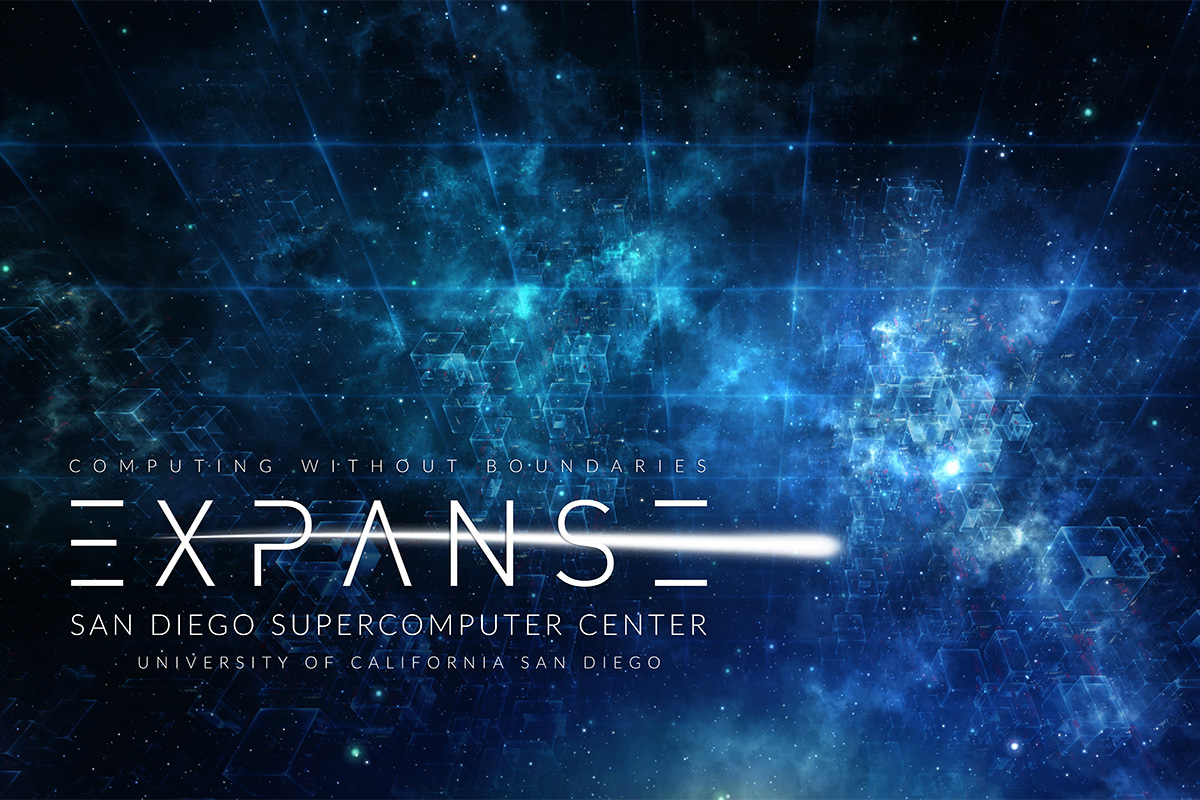
\includegraphics[width=0.7\textwidth]{expanse_logo.png}

  \end{center}
  \end{columns}
\end{frame}

\begin{frame}{Future Work: Domain Boundaries}
  \begin{columns}
  \column{0.58\linewidth}
  \begin{outline}
    \1 Spatially varying stencils 
    \1 Boundary between regions
    \1 Requires two direct solves in lock step
    \1 Would radically change plan execution
    \1 OR could use asynchronous execution
  \end{outline}

  \column{0.38\linewidth}
  \begin{center}
  \centering
  %\shadowimage[width=2.5cm]{ahmad2023_image.png}
  Filler
  \end{center}
  \end{columns}
\end{frame}

\begin{frame}{Current Work: Time Varying stencils}
  %\begin{columns}
  %\column{0.58\linewidth}
  \begin{outline}
    \1 Combine multiple stencils
    \1 Use FFT for polynomial multiplication
    \1 Use tree for lookup
  \end{outline}

  %\column{0.38\linewidth}
  
  %\end{columns}
\end{frame}
